\chapter{Recursion}

\textit{Difficult topic}
\vspace{6mm}

Recursive functions are those which call themselves again inside their function body, for example, the \texttt{fact} function that I will introduce down the chapter.

It might be difficult to get right and understand at first for learners, but it simplifies code once you get used to it. The best way to master it is through looking at more examples. You can see more examples on recursion in the mycodeschool playlist.

\section{Further resources (Ch 4-6)}

Playlists by 
\href{https://www.youtube.com/user/mycodeschool}{mycodeschool}\footnote{Link: \href{https://www.youtube.com/user/mycodeschool}{https://www.youtube.com/user/mycodeschool}}
that focus on 
\href{https://www.youtube.com/playlist?list=PL2\_aWCzGMAwLz3g66WrxFGSXvSsvyfzCO}{recursion}\footnote{Link: \href{https://www.youtube.com/playlist?list=PL2\_aWCzGMAwLz3g66WrxFGSXvSsvyfzCO}{https://www.youtube.com/playlist?list=PL2\_aWCzGMAwLz3g66WrxFGSXvSsvyfzCO}}, 
\href{https://youtube.com/playlist?list=PL2_aWCzGMAwLZp6LMUKI3cc7pgGsasm2_}{pointers}\footnote{Link: \href{https://youtube.com/playlist?list=PL2_aWCzGMAwLZp6LMUKI3cc7pgGsasm2_}{https://youtube.com/playlist?list=PL2\_aWCzGMAwLZp6LMUKI3cc7pgGsasm2\_}} and 
\href{https://www.youtube.com/playlist?list=PL2_aWCzGMAwI3W_JlcBbtYTwiQSsOTa6P}{data structures (linked lists, stacks, queues)}\footnote{Link: \href{https://www.youtube.com/playlist?list=PL2_aWCzGMAwI3W_JlcBbtYTwiQSsOTa6P}{https://www.youtube.com/playlist?list=PL2\_aWCzGMAwI3W\_JlcBbtYTwiQSsOTa6P}}.
mycodeschool explains concepts about computing pretty well. You can also watch his other playlists if interested.

\section{Example: Factorial function}

In \cref{sec:functions}, we wrote a non-recursive function that calculates the factorial of a number.
\begin{lstlisting}
int fact(int x){
    int y = 1;
    for(int i = 1; i <= x; i++){
        y *= i;
    }
    return y;
}
\end{lstlisting}

Here is an equivalent function that is recursive.

\begin{lstlisting}
int fact(int x){
    if(x==0) return 1; //0! = 1
    else return x*fact(x-1); //x! = x*(x-1)!
}
\end{lstlisting}

Let's analyse the recursive version of the function. Because it is simple\footnote{Out of scope: I call a function "simple" in this chapter if it does not invoke any side effects, such as printing something on the screen or accessing (read or write) the value of global variables. The definition is intentionally hidden for easier understanding.} we can use an equational method to analyse the function. For example, we can analyse the return value of \texttt{fact(4)} as follows:

\textit{To think about: What happens if we enter a negative number to both functions?}

\section{Example: Exponentiation}

Here is a recursive function to calculate $x^n$. \textit{Exercise: Implement a non-recursive version of the function.}

\begin{lstlisting}
int exp(int x, int n){
    if(n == 0) return 0; //x^0 = 1
    else return x*exp(x,n-1); //x^n = x*x^(n-1)
}
\end{lstlisting}

The analysis is similar to the factorial function. Here is an example of examining what \texttt{exp(2,5)} will return.

\begin{lstlisting}
exp(2,5)
= 2*exp(2,4)            (by the else clause of exp)
= 2*2*exp(2,3)          (by the else clause of exp)
= 2*2*2*exp(2,2)        (by the else clause of exp)
= 2*2*2*2*exp(2,1)      (by the else clause of exp)
= 2*2*2*2*2*exp(2,0)    (by the else clause of exp)
= 2*2*2*2*2*1           (by the if clause of exp)
= 32                    (just arithmetic)
\end{lstlisting}

\section{Example: Fast Exponentiation}

The above method of calculating $x^n$ works but it is inefficient (linear in $n$, i.e. $O(n)$, see \cref{sec:bigO}). 

People figured out a more efficient way of calculating $x^n$ (logarithmic in $n$, i.e. $O(\log n)$, see \cref{sec:bigO}). 

The mathematical formula is as follows:

\[
    x^n = \begin{cases}
    x, & \text{for } n = 1 \\
    (x^2)^{\frac{n}{2}}, & \text{for even } n \\
    x \times x^{n-1} & \text{for odd } n \neq 1\\
    \end{cases}
\]

% \begin{center}
% $x^1 = x$

% $x^{2n} = (x^2)^n$

% $x^{2n+1} = x \times (x^2)^n$
% \end{center}

For example, $2^{10} = 4^5 = 4\times 16^2 = 4\times 256 = 1024$.

The recursive code is as follows: \textit{Exercise: Implement a non-recursive version of the function.}

\begin{lstlisting}
int fastExp(int x, int n){
    if(n == 1) return x; //x^1 = x
    else if(n%2==0) return fastExp(x*x, n/2); 
        //x^n = (x*x)^(n/2) for even n
    else return x*fastExp(x*x,n/2); 
        //x^n = x*(x*x)^((n-1)/2) for odd n (n/2 is automatically rounded down in C++)
}
\end{lstlisting}

\section{Call stack}

Not every recursive function can be analysed in this way.\footnote{Out of scope: Because some functions are not "simple", that is, they invoke side effects.} To know more about recursive functions we need to learn about how functions are treated in computer memory. Internally, there is a \textbf{call stack}\index{call stack} that stores information about each function call (e.g. the values of the variables, what is left to do) so that they could resume in order.

The figure shows what happens when I call \texttt{fact(4)}.

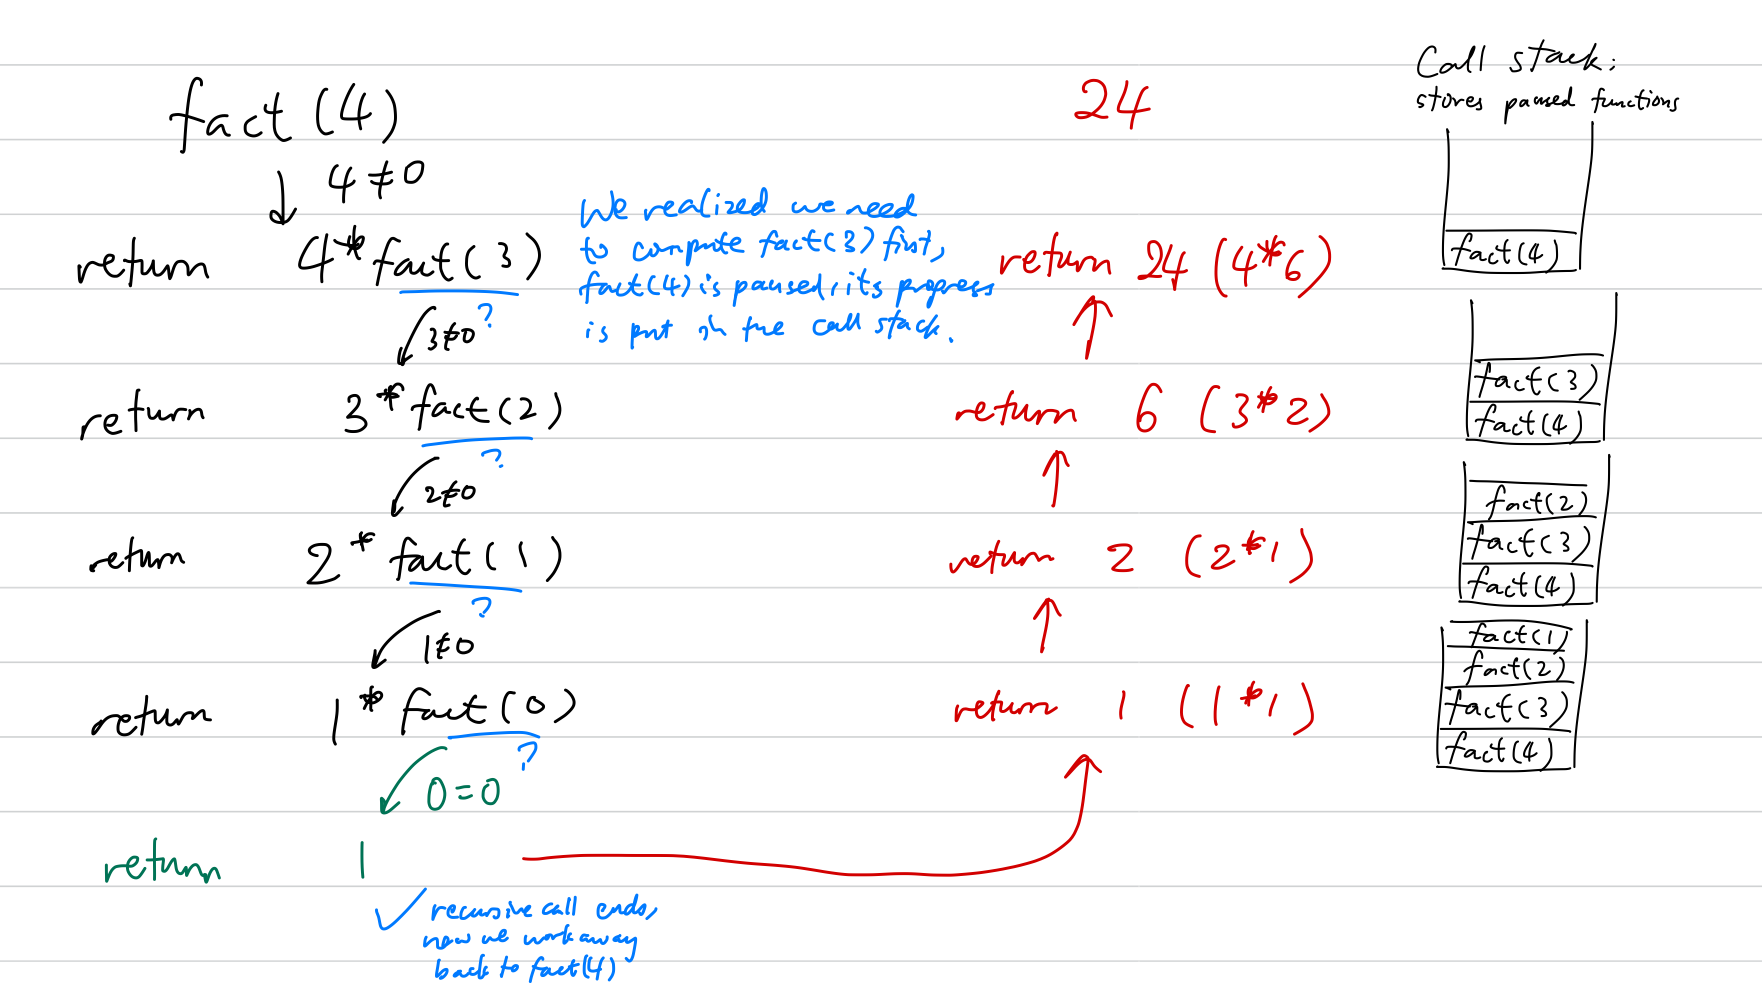
\includegraphics[width=15cm]{ch4-factorial.png}

\texttt{fact(4)} is called, realizing it needs \texttt{fact(3)} to finish, the program pauses \texttt{fact(4)}, and puts it in the call stack, so that it remembers to resume it after getting the result of \texttt{fact(3)}. A similar process happened for \texttt{fact(3)}, \texttt{fact(2)} and \texttt{fact(1)}. Finally, when \texttt{fact(0)} is called, there is no need to rely on other function calls to obtain the return value 1. We call \texttt{fact(0)} the \textbf{base case}\index{base case}. With the result of \texttt{fact(0)}, \texttt{fact(1)} can be resumed, \texttt{fact(1)} is removed from the call stack and its result is computed. A similar process happened for \texttt{fact(2)}, \texttt{fact(3)} and \texttt{fact(4)}, giving the required result finally.
\vspace{6mm}

\section{Example: Weird function}

We would use the call stack method to analyse the output of \texttt{f(0)}\footnote{Modified from HKOI 2022 Heat Senior Group \url{https://assets.hkoi.org/ref/2022hs.pdf}} . You can see the equational method does not work\footnote{Out of scope: because it involves accessing (reading and writing) the array \texttt{a}, this counts as a side effect.}.

\begin{lstlisting}
int a[7] = {3, 6, 8, 2, 5, 1, 2};
int f(int x) {
    if (x >= 3)
        return a[x];
    else {
        a[x] += f(x + 1);
        a[x] += f(x + 2);
        return a[x];
    }
}
int main() {
    cout << f(0);
    return 0;
} 
\end{lstlisting}

This kind of non-simple functions occur frequently in programming competitions but they are of less importance in university.\footnote{Recursive functions with side effects are less mathematically pleasing.}

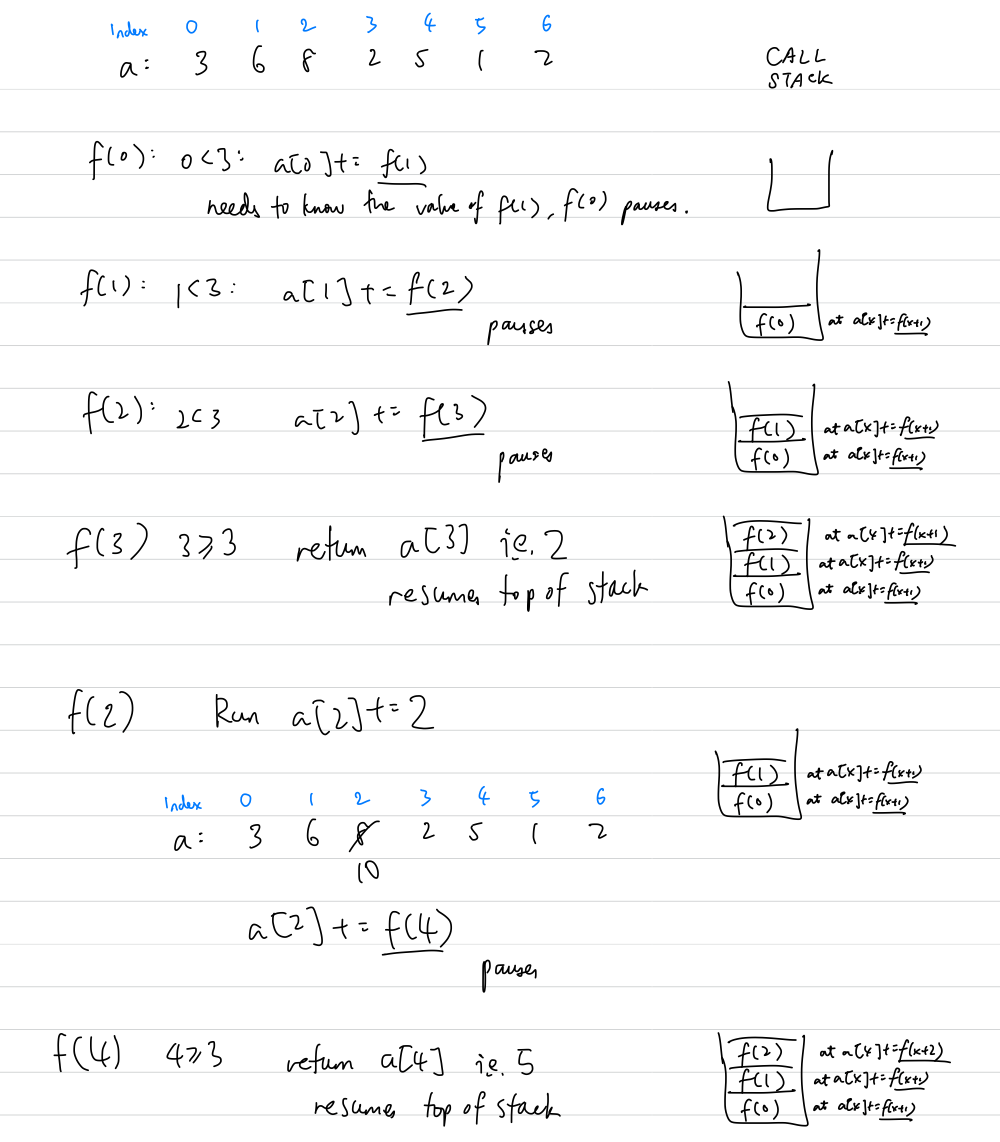
\includegraphics[width=15cm]{images/ch4-rec1.png}

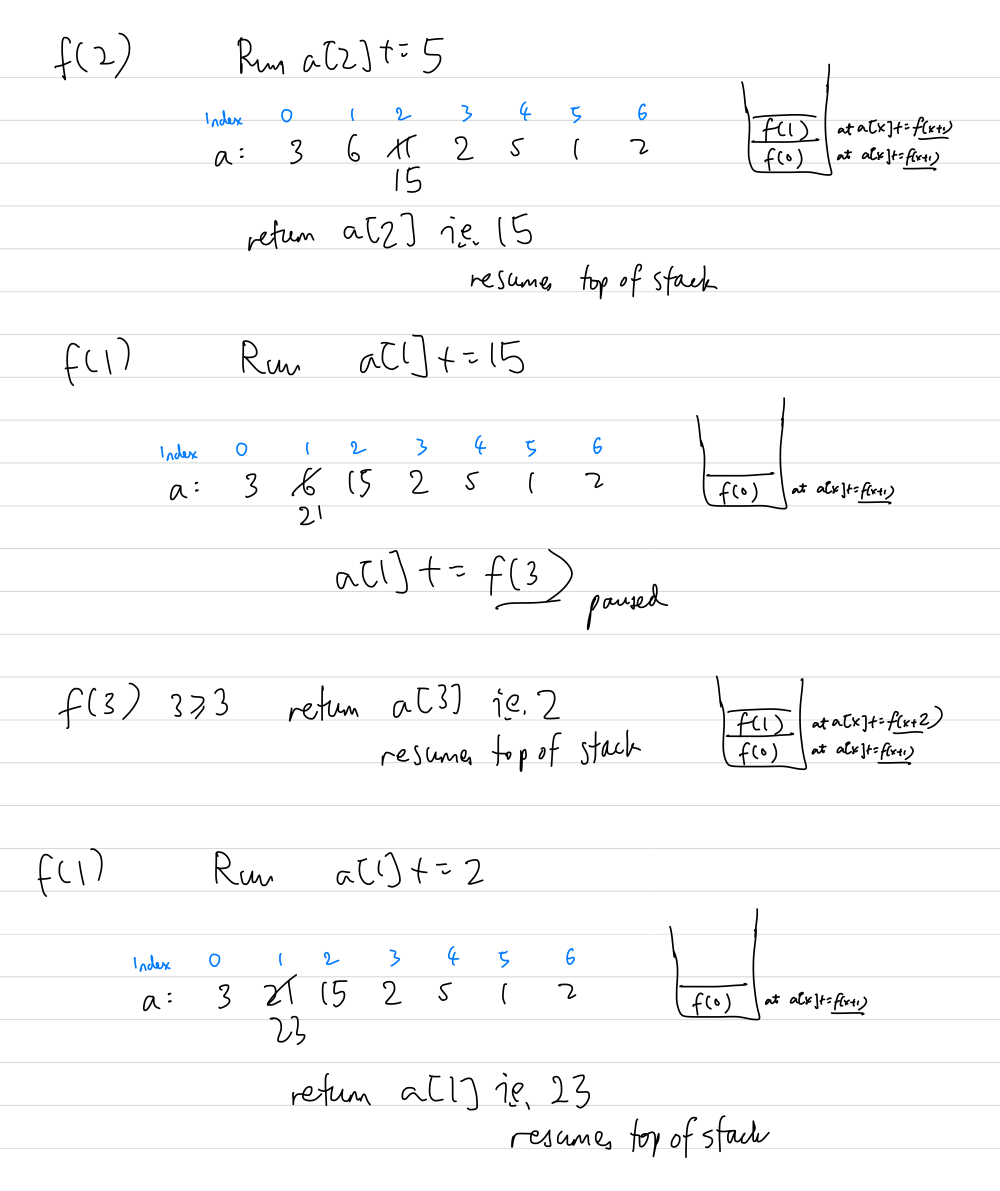
\includegraphics[width=15cm]{images/ch4-rec2.png}

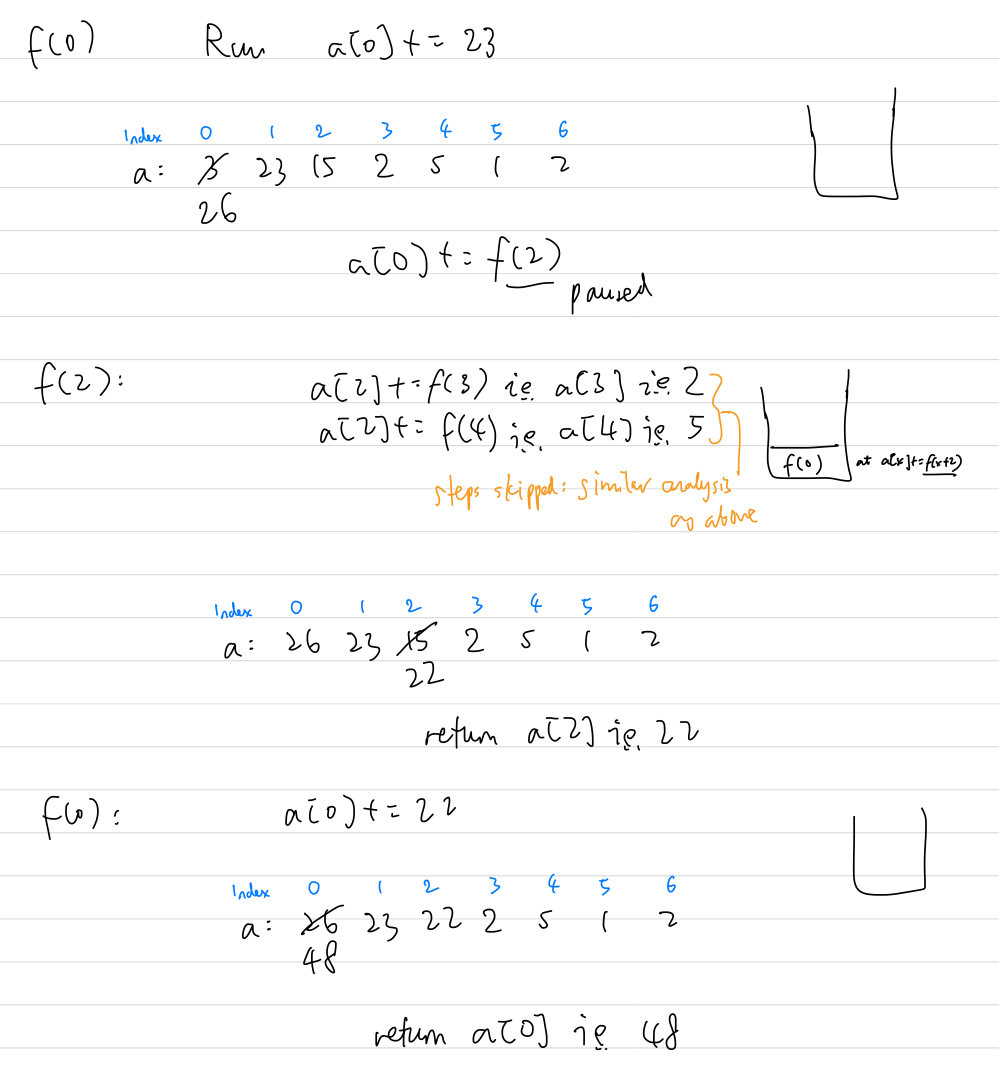
\includegraphics[width=15cm]{images/ch4-rec3.png}